\documentclass[10pt, letterpaper, titlepage]{article}
% \documentclass[10pt, letterpaper, titlepage]{report}

% % Packages
\usepackage{amsmath, amssymb, amsthm}
\usepackage{graphicx} % \dotp
\usepackage{actuarialsymbol} % \actsymb[sub][sup]{}{sub}{sup}
\usepackage{bm} % Bold text in math enviroment, \bm{}
\usepackage{xcolor} % Colored text
\usepackage{multicol} % Multiple columns, \begin{multicols}{2}
\usepackage{listings} % For displaying code
\usepackage{lplfitch} % Fitch-style proofs and Logic notations
\usepackage{url} % for \url{} if not using hyperref

\usepackage{geometry} % Margins and stuff
\usepackage{fancyhdr}

% Quattrocento font
\usepackage[sfdefault]{quattrocento}
\usepackage{lmodern} % Fixes font size
% Proofs 
\theoremstyle{definition} % no italic
\newtheorem{lemma}{Lemma}
\newtheorem{theorem}{Theorem}
\newtheorem{corollary}{Corollary}
\newtheorem{proposition}{Proposition}

% Augmented Matrix
\newenvironment{amatrix}[1]{%
  \left[\begin{array}{@{}*{#1}{c}|c@{}}
}{%
  \end{array}\right]
}

% Evaluate for calc
\newcommand*\eval[3]{\left.#1\right\rvert_{#2}^{#3}}

% Absolute Value
\newcommand*\abs[1]{\left|#1\right|}

% Floor and Ceiling function
\newcommand*\floor[1]{\left\lfloor #1 \right\rfloor}
\newcommand*\ceil[1]{\left\lceil #1 \right\rceil}

% Vector
\newcommand*\vectorvalue[1]{\langle #1 \rangle}
\newcommand*\magnitude[1]{\lVert #1 \rVert}

\makeatletter % Dot Product
\newcommand*\dotp{\mathpalette\dotp@{.5}}
\newcommand*\dotp@[2]{\mathbin{\vcenter{\hbox{\scalebox{#2}{$\m@th#1\bullet$}}}}}
\makeatother % https://tex.stackexchange.com/questions/235118/making-a-thicker-cdot-for-dot-product-that-is-thinner-than-bullet

% Sets
\newcommand*\set[1]{\{ #1 \}}
\let\intersection\cap
\let\union\cup
\let\bigintersection\bigcap
\let\bigunion\bigcup
\let\defaultemptyset\emptyset
\let\emptyset\varnothing % Nice empty sets 

% Set notations
\newcommand{\N}{\mathbb{N}} % Natural
\newcommand{\Z}{\mathbb{Z}} % Integer
\newcommand{\Q}{\mathbb{Q}} % Rational
\newcommand{\R}{\mathbb{R}} % Real
\newcommand{\C}{\mathbb{C}} % Complex
\newcommand{\Nz}{\N \union \set{0}} % Natural including 0

% Lazy
\let\e\epsilon
\newcommand*{\lhopital}{L'H\^opital}

% Logic
\newcommand{\llra}{\longleftrightarrow}

% Congruence modulo
\newcommand{\cmod}[2]{\equiv #1 \ (\mathrm{mod}\ #2)}

% For metavariables
%\usepackage[cal=boondoxo]{mathalfa}
\newcommand{\meta}[1]{\mathcal{#1}}

% Functions
\newcommand*{\sub}{\textrm{sub}} % limits of all subsequences
\newcommand*{\interior}{\textrm{int}}
\newcommand*{\bd}{\textrm{bd}} % Boundary

\newcommand*{\curl}{\textrm{curl}} % Surface Integral
\newcommand*{\divergence}{\textrm{div}} 

% Stats
\newcommand*{\E}{\textrm{E}}
\newcommand*{\Var}{\textrm{Var}}
\newcommand*{\Cov}{\textrm{Cov}}

% Finance
\newcommand*{\PA}{\textrm{PA}}
% Change lable to letter from number
\renewcommand{\thesubsection}{\alph{subsection}}

% Paragraph setup
\usepackage{parskip}
\setlength\parindent{0pt}

% Size of section header
\usepackage{sectsty}
\chaptertitlefont{\fontsize{17}{0}\selectfont}
\sectionfont{\fontsize{11}{13}\selectfont}
\subsectionfont{\fontsize{10}{12}\selectfont}
\subsubsectionfont{\fontsize{10}{12}\selectfont}

% \usepackage{hyperref} % Doesn't like math in section titles
% \newcommand{\smath}[2]{\texorpdfstring{#1}{#2}} % Use this to not break hyperref

% \setcounter{secnumdepth}{-1} % Sets sectioning level for numbering 
% % -1 part     1 section     3 subsubsection  5 subparagraph
% %  0 chapter  2 subsection  4 paragraph

% % Debug
% % For \hbox too wide errors.
% \overfullrule=.01cm

% Header
\geometry{margin = 1in}
\pagestyle{fancy}
\headheight = 23.01503pt
\lhead{}
\rhead{Yifeng Pan
     \\Draft. Not for Submission. UCID: 30063828}

% Title page
\title{Math 355 Assignment 3}
\author{Instructor: Dr Ryan Hamilton
    \\Name: Yifeng Pan
    \\UCID: 30063828}
\date{Fall 2019}

\begin{document}
    \maketitle

    \section{A math professor is interested in the relationship between students’ performance on the
    first midterm in his class and their performance on the second midterm in his class. He
    gathers the midterm 1 and midterm 2 data for his $n = 112$ students (this data is called
    “Midterm1” and “Midterm2” respectively in the “Bonus Assignment Data” R file). Note that
    the scores for both midterm 1 and midterm 2 are out of $100$ points.}
    \begin{multicols}{2}
        \subsection{Creat a scatterplot of the data. Describe the general relationship (trend) 
            of the midterm 1 and midterm 2 scores.}
            %See figure \ref{fig:1a} on page \pageref{fig:1a}.
            \begin{center}  
                % Created by tikzDevice version 0.12.3 on 2019-08-18 06:14:07
% !TEX encoding = UTF-8 Unicode
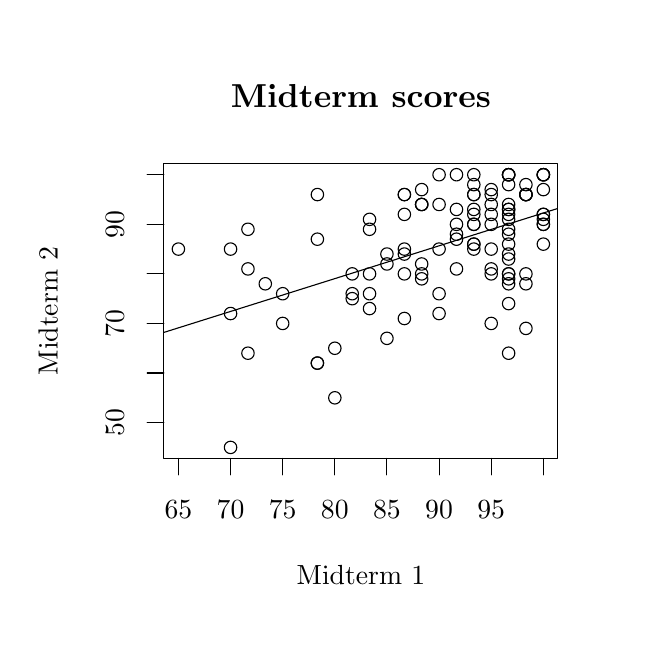
\begin{tikzpicture}[x=1pt,y=1pt]
\definecolor{fillColor}{RGB}{255,255,255}
\path[use as bounding box,fill=fillColor,fill opacity=0.00] (0,0) rectangle (216.81,216.81);
\begin{scope}
\path[clip] ( 49.20, 61.20) rectangle (191.61,167.61);
\definecolor{drawColor}{RGB}{0,0,0}

\path[draw=drawColor,line width= 0.4pt,line join=round,line cap=round] (123.53,127.84) circle (  2.25);

\path[draw=drawColor,line width= 0.4pt,line join=round,line cap=round] (180.04,156.50) circle (  2.25);

\path[draw=drawColor,line width= 0.4pt,line join=round,line cap=round] ( 92.15,109.93) circle (  2.25);

\path[draw=drawColor,line width= 0.4pt,line join=round,line cap=round] (154.95,140.38) circle (  2.25);

\path[draw=drawColor,line width= 0.4pt,line join=round,line cap=round] (173.79,151.13) circle (  2.25);

\path[draw=drawColor,line width= 0.4pt,line join=round,line cap=round] (167.50,129.63) circle (  2.25);

\path[draw=drawColor,line width= 0.4pt,line join=round,line cap=round] (136.12,156.50) circle (  2.25);

\path[draw=drawColor,line width= 0.4pt,line join=round,line cap=round] ( 54.47,136.80) circle (  2.25);

\path[draw=drawColor,line width= 0.4pt,line join=round,line cap=round] (186.34,163.67) circle (  2.25);

\path[draw=drawColor,line width= 0.4pt,line join=round,line cap=round] (186.34,138.59) circle (  2.25);

\path[draw=drawColor,line width= 0.4pt,line join=round,line cap=round] (110.99,100.97) circle (  2.25);

\path[draw=drawColor,line width= 0.4pt,line join=round,line cap=round] (142.37,127.84) circle (  2.25);

\path[draw=drawColor,line width= 0.4pt,line join=round,line cap=round] (173.79,151.13) circle (  2.25);

\path[draw=drawColor,line width= 0.4pt,line join=round,line cap=round] (173.79,143.96) circle (  2.25);

\path[draw=drawColor,line width= 0.4pt,line join=round,line cap=round] (148.66,163.67) circle (  2.25);

\path[draw=drawColor,line width= 0.4pt,line join=round,line cap=round] (173.79,163.67) circle (  2.25);

\path[draw=drawColor,line width= 0.4pt,line join=round,line cap=round] (136.12,127.84) circle (  2.25);

\path[draw=drawColor,line width= 0.4pt,line join=round,line cap=round] (161.21,160.09) circle (  2.25);

\path[draw=drawColor,line width= 0.4pt,line join=round,line cap=round] (110.99, 83.06) circle (  2.25);

\path[draw=drawColor,line width= 0.4pt,line join=round,line cap=round] (154.95,151.13) circle (  2.25);

\path[draw=drawColor,line width= 0.4pt,line join=round,line cap=round] (180.04,108.14) circle (  2.25);

\path[draw=drawColor,line width= 0.4pt,line join=round,line cap=round] (136.12,136.80) circle (  2.25);

\path[draw=drawColor,line width= 0.4pt,line join=round,line cap=round] (129.82,104.55) circle (  2.25);

\path[draw=drawColor,line width= 0.4pt,line join=round,line cap=round] (136.12,135.01) circle (  2.25);

\path[draw=drawColor,line width= 0.4pt,line join=round,line cap=round] (167.50,145.75) circle (  2.25);

\path[draw=drawColor,line width= 0.4pt,line join=round,line cap=round] (123.53,143.96) circle (  2.25);

\path[draw=drawColor,line width= 0.4pt,line join=round,line cap=round] (173.79,127.84) circle (  2.25);

\path[draw=drawColor,line width= 0.4pt,line join=round,line cap=round] (117.28,127.84) circle (  2.25);

\path[draw=drawColor,line width= 0.4pt,line join=round,line cap=round] (180.04,127.84) circle (  2.25);

\path[draw=drawColor,line width= 0.4pt,line join=round,line cap=round] (186.34,149.34) circle (  2.25);

\path[draw=drawColor,line width= 0.4pt,line join=round,line cap=round] (167.50,127.84) circle (  2.25);

\path[draw=drawColor,line width= 0.4pt,line join=round,line cap=round] (161.21,138.59) circle (  2.25);

\path[draw=drawColor,line width= 0.4pt,line join=round,line cap=round] (154.95,142.17) circle (  2.25);

\path[draw=drawColor,line width= 0.4pt,line join=round,line cap=round] (142.37,126.05) circle (  2.25);

\path[draw=drawColor,line width= 0.4pt,line join=round,line cap=round] (180.04,156.50) circle (  2.25);

\path[draw=drawColor,line width= 0.4pt,line join=round,line cap=round] (161.21,145.75) circle (  2.25);

\path[draw=drawColor,line width= 0.4pt,line join=round,line cap=round] (180.04,160.09) circle (  2.25);

\path[draw=drawColor,line width= 0.4pt,line join=round,line cap=round] (161.21,151.13) circle (  2.25);

\path[draw=drawColor,line width= 0.4pt,line join=round,line cap=round] (129.82,131.42) circle (  2.25);

\path[draw=drawColor,line width= 0.4pt,line join=round,line cap=round] (142.37,158.29) circle (  2.25);

\path[draw=drawColor,line width= 0.4pt,line join=round,line cap=round] (186.34,163.67) circle (  2.25);

\path[draw=drawColor,line width= 0.4pt,line join=round,line cap=round] (180.04,156.50) circle (  2.25);

\path[draw=drawColor,line width= 0.4pt,line join=round,line cap=round] (173.79,117.09) circle (  2.25);

\path[draw=drawColor,line width= 0.4pt,line join=round,line cap=round] (148.66,136.80) circle (  2.25);

\path[draw=drawColor,line width= 0.4pt,line join=round,line cap=round] (136.12,156.50) circle (  2.25);

\path[draw=drawColor,line width= 0.4pt,line join=round,line cap=round] (186.34,145.75) circle (  2.25);

\path[draw=drawColor,line width= 0.4pt,line join=round,line cap=round] (173.79,152.92) circle (  2.25);

\path[draw=drawColor,line width= 0.4pt,line join=round,line cap=round] (180.04,156.50) circle (  2.25);

\path[draw=drawColor,line width= 0.4pt,line join=round,line cap=round] (148.66,152.92) circle (  2.25);

\path[draw=drawColor,line width= 0.4pt,line join=round,line cap=round] (173.79,142.17) circle (  2.25);

\path[draw=drawColor,line width= 0.4pt,line join=round,line cap=round] (136.12,149.34) circle (  2.25);

\path[draw=drawColor,line width= 0.4pt,line join=round,line cap=round] (167.50,136.80) circle (  2.25);

\path[draw=drawColor,line width= 0.4pt,line join=round,line cap=round] (104.69, 95.60) circle (  2.25);

\path[draw=drawColor,line width= 0.4pt,line join=round,line cap=round] (136.12,111.72) circle (  2.25);

\path[draw=drawColor,line width= 0.4pt,line join=round,line cap=round] (186.34,158.29) circle (  2.25);

\path[draw=drawColor,line width= 0.4pt,line join=round,line cap=round] (117.28,120.67) circle (  2.25);

\path[draw=drawColor,line width= 0.4pt,line join=round,line cap=round] (173.79,126.05) circle (  2.25);

\path[draw=drawColor,line width= 0.4pt,line join=round,line cap=round] (154.95,163.67) circle (  2.25);

\path[draw=drawColor,line width= 0.4pt,line join=round,line cap=round] (173.79,135.01) circle (  2.25);

\path[draw=drawColor,line width= 0.4pt,line join=round,line cap=round] (173.79,163.67) circle (  2.25);

\path[draw=drawColor,line width= 0.4pt,line join=round,line cap=round] (167.50,152.92) circle (  2.25);

\path[draw=drawColor,line width= 0.4pt,line join=round,line cap=round] (173.79,160.09) circle (  2.25);

\path[draw=drawColor,line width= 0.4pt,line join=round,line cap=round] ( 85.86,124.26) circle (  2.25);

\path[draw=drawColor,line width= 0.4pt,line join=round,line cap=round] (186.34,145.75) circle (  2.25);

\path[draw=drawColor,line width= 0.4pt,line join=round,line cap=round] (161.21,138.59) circle (  2.25);

\path[draw=drawColor,line width= 0.4pt,line join=round,line cap=round] (173.79,133.21) circle (  2.25);

\path[draw=drawColor,line width= 0.4pt,line join=round,line cap=round] (142.37,152.92) circle (  2.25);

\path[draw=drawColor,line width= 0.4pt,line join=round,line cap=round] ( 73.31, 65.14) circle (  2.25);

\path[draw=drawColor,line width= 0.4pt,line join=round,line cap=round] (173.79,138.59) circle (  2.25);

\path[draw=drawColor,line width= 0.4pt,line join=round,line cap=round] (173.79, 99.18) circle (  2.25);

\path[draw=drawColor,line width= 0.4pt,line join=round,line cap=round] (186.34,149.34) circle (  2.25);

\path[draw=drawColor,line width= 0.4pt,line join=round,line cap=round] (142.37,152.92) circle (  2.25);

\path[draw=drawColor,line width= 0.4pt,line join=round,line cap=round] (173.79,163.67) circle (  2.25);

\path[draw=drawColor,line width= 0.4pt,line join=round,line cap=round] (186.34,163.67) circle (  2.25);

\path[draw=drawColor,line width= 0.4pt,line join=round,line cap=round] (142.37,131.42) circle (  2.25);

\path[draw=drawColor,line width= 0.4pt,line join=round,line cap=round] (186.34,147.55) circle (  2.25);

\path[draw=drawColor,line width= 0.4pt,line join=round,line cap=round] (104.69, 95.60) circle (  2.25);

\path[draw=drawColor,line width= 0.4pt,line join=round,line cap=round] (161.21,149.34) circle (  2.25);

\path[draw=drawColor,line width= 0.4pt,line join=round,line cap=round] (173.79,149.34) circle (  2.25);

\path[draw=drawColor,line width= 0.4pt,line join=round,line cap=round] ( 79.60,143.96) circle (  2.25);

\path[draw=drawColor,line width= 0.4pt,line join=round,line cap=round] (142.37,152.92) circle (  2.25);

\path[draw=drawColor,line width= 0.4pt,line join=round,line cap=round] ( 79.60, 99.18) circle (  2.25);

\path[draw=drawColor,line width= 0.4pt,line join=round,line cap=round] (173.79,127.84) circle (  2.25);

\path[draw=drawColor,line width= 0.4pt,line join=round,line cap=round] (161.21,156.50) circle (  2.25);

\path[draw=drawColor,line width= 0.4pt,line join=round,line cap=round] (173.79,124.26) circle (  2.25);

\path[draw=drawColor,line width= 0.4pt,line join=round,line cap=round] (167.50,158.29) circle (  2.25);

\path[draw=drawColor,line width= 0.4pt,line join=round,line cap=round] (180.04,124.26) circle (  2.25);

\path[draw=drawColor,line width= 0.4pt,line join=round,line cap=round] (104.69,140.38) circle (  2.25);

\path[draw=drawColor,line width= 0.4pt,line join=round,line cap=round] (148.66,113.51) circle (  2.25);

\path[draw=drawColor,line width= 0.4pt,line join=round,line cap=round] (173.79,147.55) circle (  2.25);

\path[draw=drawColor,line width= 0.4pt,line join=round,line cap=round] ( 79.60,129.63) circle (  2.25);

\path[draw=drawColor,line width= 0.4pt,line join=round,line cap=round] (167.50,149.34) circle (  2.25);

\path[draw=drawColor,line width= 0.4pt,line join=round,line cap=round] (123.53,120.67) circle (  2.25);

\path[draw=drawColor,line width= 0.4pt,line join=round,line cap=round] (148.66,120.67) circle (  2.25);

\path[draw=drawColor,line width= 0.4pt,line join=round,line cap=round] (173.79,163.67) circle (  2.25);

\path[draw=drawColor,line width= 0.4pt,line join=round,line cap=round] (123.53,115.30) circle (  2.25);

\path[draw=drawColor,line width= 0.4pt,line join=round,line cap=round] (186.34,163.67) circle (  2.25);

\path[draw=drawColor,line width= 0.4pt,line join=round,line cap=round] (123.53,147.55) circle (  2.25);

\path[draw=drawColor,line width= 0.4pt,line join=round,line cap=round] (104.69,156.50) circle (  2.25);

\path[draw=drawColor,line width= 0.4pt,line join=round,line cap=round] (161.21,156.50) circle (  2.25);

\path[draw=drawColor,line width= 0.4pt,line join=round,line cap=round] (117.28,118.88) circle (  2.25);

\path[draw=drawColor,line width= 0.4pt,line join=round,line cap=round] (161.21,163.67) circle (  2.25);

\path[draw=drawColor,line width= 0.4pt,line join=round,line cap=round] (154.95,145.75) circle (  2.25);

\path[draw=drawColor,line width= 0.4pt,line join=round,line cap=round] (161.21,136.80) circle (  2.25);

\path[draw=drawColor,line width= 0.4pt,line join=round,line cap=round] ( 92.15,120.67) circle (  2.25);

\path[draw=drawColor,line width= 0.4pt,line join=round,line cap=round] ( 73.31,136.80) circle (  2.25);

\path[draw=drawColor,line width= 0.4pt,line join=round,line cap=round] (129.82,135.01) circle (  2.25);

\path[draw=drawColor,line width= 0.4pt,line join=round,line cap=round] ( 73.31,113.51) circle (  2.25);

\path[draw=drawColor,line width= 0.4pt,line join=round,line cap=round] (154.95,129.63) circle (  2.25);

\path[draw=drawColor,line width= 0.4pt,line join=round,line cap=round] (161.21,145.75) circle (  2.25);

\path[draw=drawColor,line width= 0.4pt,line join=round,line cap=round] (167.50,109.93) circle (  2.25);

\path[draw=drawColor,line width= 0.4pt,line join=round,line cap=round] (167.50,156.50) circle (  2.25);
\end{scope}
\begin{scope}
\path[clip] (  0.00,  0.00) rectangle (216.81,216.81);
\definecolor{drawColor}{RGB}{0,0,0}

\path[draw=drawColor,line width= 0.4pt,line join=round,line cap=round] ( 54.47, 61.20) -- (186.34, 61.20);

\path[draw=drawColor,line width= 0.4pt,line join=round,line cap=round] ( 54.47, 61.20) -- ( 54.47, 55.20);

\path[draw=drawColor,line width= 0.4pt,line join=round,line cap=round] ( 73.31, 61.20) -- ( 73.31, 55.20);

\path[draw=drawColor,line width= 0.4pt,line join=round,line cap=round] ( 92.15, 61.20) -- ( 92.15, 55.20);

\path[draw=drawColor,line width= 0.4pt,line join=round,line cap=round] (110.99, 61.20) -- (110.99, 55.20);

\path[draw=drawColor,line width= 0.4pt,line join=round,line cap=round] (129.82, 61.20) -- (129.82, 55.20);

\path[draw=drawColor,line width= 0.4pt,line join=round,line cap=round] (148.66, 61.20) -- (148.66, 55.20);

\path[draw=drawColor,line width= 0.4pt,line join=round,line cap=round] (167.50, 61.20) -- (167.50, 55.20);

\path[draw=drawColor,line width= 0.4pt,line join=round,line cap=round] (186.34, 61.20) -- (186.34, 55.20);

\node[text=drawColor,anchor=base,inner sep=0pt, outer sep=0pt, scale=  1.00] at ( 54.47, 39.60) {65};

\node[text=drawColor,anchor=base,inner sep=0pt, outer sep=0pt, scale=  1.00] at ( 73.31, 39.60) {70};

\node[text=drawColor,anchor=base,inner sep=0pt, outer sep=0pt, scale=  1.00] at ( 92.15, 39.60) {75};

\node[text=drawColor,anchor=base,inner sep=0pt, outer sep=0pt, scale=  1.00] at (110.99, 39.60) {80};

\node[text=drawColor,anchor=base,inner sep=0pt, outer sep=0pt, scale=  1.00] at (129.82, 39.60) {85};

\node[text=drawColor,anchor=base,inner sep=0pt, outer sep=0pt, scale=  1.00] at (148.66, 39.60) {90};

\node[text=drawColor,anchor=base,inner sep=0pt, outer sep=0pt, scale=  1.00] at (167.50, 39.60) {95};

\path[draw=drawColor,line width= 0.4pt,line join=round,line cap=round] ( 49.20, 74.10) -- ( 49.20,163.67);

\path[draw=drawColor,line width= 0.4pt,line join=round,line cap=round] ( 49.20, 74.10) -- ( 43.20, 74.10);

\path[draw=drawColor,line width= 0.4pt,line join=round,line cap=round] ( 49.20, 92.01) -- ( 43.20, 92.01);

\path[draw=drawColor,line width= 0.4pt,line join=round,line cap=round] ( 49.20,109.93) -- ( 43.20,109.93);

\path[draw=drawColor,line width= 0.4pt,line join=round,line cap=round] ( 49.20,127.84) -- ( 43.20,127.84);

\path[draw=drawColor,line width= 0.4pt,line join=round,line cap=round] ( 49.20,145.75) -- ( 43.20,145.75);

\path[draw=drawColor,line width= 0.4pt,line join=round,line cap=round] ( 49.20,163.67) -- ( 43.20,163.67);

\node[text=drawColor,rotate= 90.00,anchor=base,inner sep=0pt, outer sep=0pt, scale=  1.00] at ( 34.80, 74.10) {50};

\node[text=drawColor,rotate= 90.00,anchor=base,inner sep=0pt, outer sep=0pt, scale=  1.00] at ( 34.80,109.93) {70};

\node[text=drawColor,rotate= 90.00,anchor=base,inner sep=0pt, outer sep=0pt, scale=  1.00] at ( 34.80,145.75) {90};

\path[draw=drawColor,line width= 0.4pt,line join=round,line cap=round] ( 49.20, 61.20) --
	(191.61, 61.20) --
	(191.61,167.61) --
	( 49.20,167.61) --
	( 49.20, 61.20);
\end{scope}
\begin{scope}
\path[clip] (  0.00,  0.00) rectangle (216.81,216.81);
\definecolor{drawColor}{RGB}{0,0,0}

\node[text=drawColor,anchor=base,inner sep=0pt, outer sep=0pt, scale=  1.20] at (120.41,188.07) {\bfseries Midterm scores};

\node[text=drawColor,anchor=base,inner sep=0pt, outer sep=0pt, scale=  1.00] at (120.41, 15.60) {Midterm 1};

\node[text=drawColor,rotate= 90.00,anchor=base,inner sep=0pt, outer sep=0pt, scale=  1.00] at ( 10.80,114.41) {Midterm 2};
\end{scope}
\begin{scope}
\path[clip] ( 49.20, 61.20) rectangle (191.61,167.61);
\definecolor{drawColor}{RGB}{0,0,0}

\path[draw=drawColor,line width= 0.4pt,line join=round,line cap=round] ( 49.20,106.68) -- (191.61,151.50);
\end{scope}
\end{tikzpicture}

            \end{center}

        \subsection{What is the correlation between midterm 1 grades and midterm 2 grades? Interpret
            this correlation.}
            $r \approx 0.5048535$

        \subsection{State the least-squares estimate of the model predicting midterm 2 scores from
            midterm 1 scores.}
            $m_2 \approx 0.6619698m_1 + 26.0843211$

        \subsection{Interpret the slope of this regression equation in the context of the data.}
            For every 1 point increase on a student's score on midterm 1, 
            there will be a 0.6620 point increase on the student's score on midterm 2.

        \subsection{Predict the midterm 2 score of a student who scored 60 on midterm 1.}
            $m_2 \approx 0.6619698m_1 + 26.0843211$\\
            $= 0.6619698(60) + 26.0843211 \approx 65.80$

        \subsection{Predict the midterm 2 score of a student who scored 92 on midterm 1.}
            $m_2 \approx 0.6619698m_1 + 26.0843211$\\
            $= 0.6619698(92) + 26.0843211 \approx 86.99$

        \subsection{Suppose a student scored a 80 on\\
            midterm 1. Calculate the residual for this student if
            they also scored an 80 on midterm 2.}
            $\epsilon = m_2 - \hat m_2 \approx 80 - (0.6619698m_1 + 26.0843211)$\\
            $= 80 - (0.6619698(80) + 26.0843211) \approx 0.9581$

        \subsection{Assuming the normality condition is met, what would you expect the normal
            probability plot of the residuals to look like? Describe it in words or draw a picture.}
            See figure \ref{fig:1h} on page \pageref{fig:1h}.\\
            The historgram is close to normal. 
            On the normal probabily plot, the dots are close to the lines.

        \subsection{Conduct a hypothesis test to determine if midterm 2 scores can be expressed as a linear
            function of midterm 1 scores. Please state all steps of the hypothesis testing process
            (hypotheses, test statistic, p-value, conclusion). Use $\alpha = 0.05$.}
            $H_0: \beta_1 = 0, H_a: \beta_1 \neq 0$\\
            $t = \frac{\beta_1 - \beta_{1_0}}{SE_{\beta_1}} 
            \approx \frac{0.662 - 0}{0.107917} \approx 6.134$\\
            $\pv = 2 * (1 - pt(t, 110)) \approx 1.377 * 10^{-8} < 0.05 = \alpha$\\
            Therefore there is a linear dependency of the score on midterm 1
            on midterm 2.

        \subsection{Construct a $95\%$ confidence interval for the slope. Does this confidence interval suggest
            that the slope is significantly different from zero?}
            Confidence interval: (0.4481033, 0.8758362). \\
            Yes, it does not contain 0.
    \end{multicols}
    % \newpage
    \section{Is academic salary related to the number of years since the highest degree earned? A
    random sample of 52 tenure-track professors was taken. Each professor’s academic
    yearly salary (in dollars) was recorded, as well as the time (in years) since their highest
    degree had been earned (this data is called “Salary” and “Years” respectively in the
    “Bonus Assignment Data” R file).}
    \begin{multicols}{2}
        \subsection{What is the value of the coefficient of determination? Interpret its meaning in this
            context.}
            $r^2 \approx 0.4554$

        \subsection{Write down the least-squares estimate of the model predicting yearly salary from years
            since highest degree earned.}
            $s \approx 390.6y + 17500$

        \subsection{Interpret the slope of this regression equation.}
            For every 1 year increase the amount of time since highest degree earned, 
            there will be a 390.6 dollar increase in salary.

        \subsection{Interpret the y-intercept of this regression equation. Does the y-intercept have a
            “practical” (meaningful) interpretation?}
            It means the starting salary from highest degree earned is 17500 dollars.\\
            Yes

        \subsection{Predict the yearly salary for a tenure-track professor for whom there has been 29
            years since his/her highest degree was earned.}
            $s \approx 390.6451y + 17502.2574$\\
            $= 390.6451(29) + 17502.2574$
            $\approx 28830$

        \subsection{A tenure-track professor for whom there has been 29 years since his/her highest
            degree was earned is actually earning $\$22,450$ yearly. Compute this professor’s
            residual.}
            $\epsilon = s - \hat s \approx 22450 - (390.6451(29) + 17502.2574)$
            $\approx -6381$
            
        \subsection{Examine the normality plot. What condition/assumption does the normality plot check for?
            Does it appear to be met in this case?}
            See figure \ref{fig:2g} on page \pageref{fig:2g}.\\
            The normality plot checks if the data approximates a normal distro.
            In this case, it does, as the dots are close enough to the line.
            And the histogram is close enough to a bell curve.
    \end{multicols}
    \section{Suppose $f:[0,\infty) \to \R$ is continuous, monotone and bounded.
    Show that $f$ is uniformly continuous. (Hint: We know that $f([0,\infty))$ is an interval.)
}
    TODO

    % % Attempt 3

    Since $f$ is monotone and bounded, $f(n) = L$ as $n \to \infty$.

    Let $a = \min\set{f(0), L}, b = \max\set{f(0), L}$.

    From the Intermediate Value Theorem, 
    we know $\lall t \in (a,b), \lis c \in [0,\infty)$ 
    such that $f(c) = t$.

    We define $g: (a,b) \to [0,\infty)$.
    The range of $g \subseteq [0, \infty)$.
    % $g$ is monotone as $f$ is monotone. % Need more
    So $\lall y \in (a,b), f \circ g (y) = y$.

    Let $\e > 0$.

    Let $h: (a, b - \e) \to (0, \infty), h(y) = \abs{g(y) - g(y + \e)}$.
    $h$ is strictly positive. % Justify

    % Let $h_c(x,y): \set{(a,b) \times (a,b) | 0 < \abs{x-y} <c} \to (0, \infty), 
    %     h(x,y) = \abs{g(x) - g(y)}$.
    % $h$ is strictly positive. % Justify

    Let $\delta$ be the absolute minimum of the range of $h$.

    % Proof of contrapositive.

    % Let $\abs{f(x) - f(y)} \geq \e$.


    Let $x,y \in [0, \infty), \abs{x - y} < \delta$.

    So $\lall z \in (a, b - \e),\abs{x-y} < \abs{g(z) - g(z + \e)}$.

    % Proof by contradiction.

    % Suppose $\abs{f(x) - f(y)} > \e$.

    % Now,
    % \begin{align*}
    %     \abs{f(x) - f(y)}
    % \end{align*}


    % % Attempt 2
    % To Prove: $f^{-1}$ Exists.

    % Since $f$ is bounded, let $I = f([0,\infty])$ be an finite interval.
    % Let $a = \inf(I), b = \sup(I)$.
    % Let $f^{-1}: I \to [0, \infty)$.

    % Let $\e > 0$.
    % Define a finite sequence $\set{\e_n}$ such that
    % \begin{enumerate}
    %     \item $0 < \abs{\e_1 - a} < \e$.
    %     \item $0 < \abs{\e_n - b} < \e$.
    %     \item $\lall i \in \N, 1 < i <= n, \e_i = \e_{i-1} + \e$.
    % \end{enumerate}


    % % Scrap
    % Let $n = \floor{\frac{b - a}{\e'}} - 1$.
    % Define the set $S$ where 
    % $x\in S$
    % $\liff$ 
    % $\lis i \in \N, i <= n$
    % such that $x = a + i \e'$.

    % Define the set $\set{\e'_n}$ such that
    % \(
    %     \e'_i = a + i \e'
    % \)


    % % Attempt 1
    % Since $f$ is bounded, 
    % $\lis M > 0$ such that $\abs{f(x)} < M, \lall x$.

    % % Since $f$ is bounded and continuous,
    % % let $I$ be the range of $f$, by IVT.

    % Let $\e > 0$.
    % Choose $\delta = \frac{\e}{M} TODO$.
    % % Let $a,b,c \in [0,\infty), a \leq b \leq c$. 
    % Let $x,y \in [0,\infty) $, Let $a = \min\set{x,y}, c = \max\set{x,y}$.
    % Suppose $\abs{x-y} = c - a < \delta$.

    % \begin{align*}
    %     \abs{f(x) - f(y)}
    %     &= f(c) - f(a) \text{ ($f$ is monotone)} \\
    %     &< \\
    %     &TODO< \e
    % \end{align*}
    \section{Suppose $x_1, x_2, y_1, y_2$ are real numbers. Show that 
    \[x_1y_1 + x_2y_2 \leq \sqrt{x_1^2 + x_2^2}\sqrt{y_1^2 + y_2^2}
        \]
    Fully describe the set of points for which the above inequality is an equality.}
    Proof: 
    \begin{align*}
        x_1y_1 + x_2y_2 &\leq \abs{x_1y_1 + x_2y_2} \\ 
        &= \sqrt{(x_1y_1 + x_2y_2)^2} \\ 
        &= \sqrt{x_1^2y_1^2 + 2x_1y_1x_2y_2 + x_2^2y_2^2} \\ 
        &\leq \sqrt{x_1^2y_1^2 + x_2^2y_1^2 + x_1^2y_2^2 + x_2^2y_2^2} \text{ (Lemma)}\\ 
        &= \sqrt{(x_1^2 + x_2^2) (y_1^2 + y_2^2)} \\ 
        &= \sqrt{x_1^2 + x_2^2}\sqrt{y_1^2 + y_2^2} \\ 
    \end{align*}
    Lemma:

    $(\sqrt{x_1^2y_1^2 + 2x_1y_1x_2y_2 + x_2^2y_2^2} 
    \leq \sqrt{x_1^2y_1^2 + x_2^2y_1^2 + x_1^2y_2^2 + x_2^2y_2^2})$
    IFF $(2x_1y_1x_2y_2 \leq x_2^2y_1^2 + x_1^2y_2^2)$.

    Proof that $(2x_1y_1x_2y_2 \leq x_2^2y_1^2 + x_1^2y_2^2)$:
    \begin{align*}
        2x_1y_1x_2y_2
        &\leq (x_2y_1 - x_1y_2)^2 + 2x_1y_1x_2y_2 \\ 
        &= x_2^2y_1^2 + x_1^2y_2^2 - 2x_1y_1x_2y_2 + 2x_1y_1x_2y_2 \\ 
        &= x_2^2y_1^2 + x_1^2y_2^2
    \end{align*}

    Set of points: 

    Using the above proof, it's easy to see that: \\ 
    $x_1y_1 + x_2y_2 = \sqrt{x_1^2 + x_2^2}\sqrt{y_1^2 + y_2^2}$
    IFF 
    ($x_1y_1 + x_2y_2 = \abs{x_1y_1 + x_2y_2}$
    AND $2x_1y_1x_2y_2 = x_2^2y_1^2 + x_1^2y_2^2$).

    $x_1y_1 + x_2y_2 = \abs{x_1y_1 + x_2y_2}$ means $x_1y_1 + x_2y_2$ is non-negative.

    Now, 
    \begin{align*}
        2x_1y_1x_2y_2 &= x_2^2y_1^2 + x_1^2y_2^2 \\ 
        0 &= x_2^2y_1^2 + x_1^2y_2^2 - 2x_1y_1x_2y_2 \\ 
        &= (x_2y_1 - x_1y_2)^2
    \end{align*}
    Therefore $x_2y_1 - x_1y_2 = 0, x_1y_2 = x_2y_1$.

    The solutions to $x_1y_1 + x_2y_2 = \sqrt{x_1^2 + x_2^2}\sqrt{y_1^2 + y_2^2}$
    are $\set{x_1,x_2,y_1,y_2 \in \R | x_1y_1 + x_2y_2 \geq 0, x_1y_2 = x_2y_1}$.
    \section{}
    \subsection{Suppose $x < y$ are real numbers. Show that there are infinitely many distinct
        rational numbers $q$ such that $x < q < y$.}
        Let $n \in N$ such that $1/n < (y - x) / 3$ where $(y - x) / 3 \in \R$
        (corollary of the Archimedean Property).
        So $(yn - xn) > 3$.
        Therefore there are atleast two consecutive integers $i, i+1$ between $yn$ and $xn$.
        So we have $x < i/n < (i+1) / n < y$, where $i/n, (i+1)/n \in \Q$.
        Now, let $A = \set{\frac{i}{n} + \frac{1}{n + k} | k \in \N}$.
        It's easy to see that every element of $A$ is between $i/n$ and $(i + 1)/n$.
        Therefore $A$ is an infinite set of rationals between $x$ and $y$.

    \subsection{Suppose $x < y$ are real numbers. Show that there are infinitely many distinct
        irrational numbers $w$ such that $x < w < y$. Are there uncountably many?}
        Let $x, y \in \R$, such that $x < y$.
        Let $R' \subseteq \R$ be a set containing all reals between $x$ and $y$.
        Let $Q' \subseteq \Q$ be a set containing all rationals between $x$ and $y$.
        We know that $R'$ is uncountably infinite.
        And we know that $Q'$ is countable.
        Let $S = R' \setminus Q'$ be a set containing all of the irrationals between $x$ and $y$.
        Given that a uncountably infinite set minus a countable set is still uncoutably infinite,
        there are an uncountably infinite number of irrationals between $x$ and $y$.
    \section{}
    \subsection{Find an explict injection $f: \Q \to \Z$}
        Let $q \in \Q$.
        Let $a \in \Z, b \in \N$ such that $(a,b) \in \Q$ is the irreducible fraction of $q$.
            \footnote{I've been instructed to clarify the definition of "irreducible fraction", 
            I've provided an attempt on page~\pageref{proof:IF}.}
        Let $m = \max(\abs{a},b)$.
        Let $n = 10$.
        Let $d = \floor{\log_{n}(m)} + 1$ 
        (where $\floor{x}$ means floor of $x$).
        \[
            f(q) = 
            \begin{cases}
                n^{2d} + n^d a + b & \text{ if $a \geq 0$} \\ 
                -(n^{2d} + n^d \abs{a} + b) & \text{ if $a < 0$}
            \end{cases}
        \]
        It's easy to see that $f(q) \in\Z$, 
        as $n, a, b, d \in \Z, d \geq 1$.
        
        Let $f^{-1}: \{f(x) | x \in \Q \} \to \Q$.
        Let $z \in \set{f(x) | x \in \Q}$.
        Let $n = 10$.
        Let $d' = \floor{\log_n \abs{z}} / 2$.
        Let $z' = \abs{z} \mod n^{2d'}$.
        $$
            \text{Let } a' = 
            \begin{cases}
                \floor{z' n^{-d'}} &\text{ if $z \geq 0$} \\ 
                -\floor{z' n^{-d'}} &\text{ if $z < 0$}
            \end{cases}
        $$
        Let $b' = z' \mod n^{d'}$.
        \[
            f^{-1}(z) = (a',b')
        \]
        Where $(a',b') \in \Q$.
        Because there is a function from the image of $f$ to the domain of $f$,
        $f$ is injective.

        Proof that $f^{-1}(f(q)) = q, \forall q \in \Q$: \\ 
        The following is for the non-negative case, the negative case can be proven similarly. \\ 
        $f^{-1}(f(q)) = f^{-1}(n^{2d} + n^d a + b)$.
        In this case $d' = \floor{\log_n \abs{n^{2d} + n^d a + b}} / 2 = 2d / 2 = d$.
        \footnote{$a < n^d, b < n^d$ by construction, as $d = \floor{\log_n(\max(\abs{a}, b))} + 1$.}
        And $z' = (n^{2d} + n^d a + b) \mod n^{2d} = n^d a + b$.
        Then $a' = \floor{(n^d a + b) n^{-d'}} = \floor{a + b n^{-d'}} = a$.
        And $b' = (n^d a + b) \mod n^{d'} = b$.
        So $f^{-1}(f(q)) = f^{-1}(n^{2d} + n^d a + b) = (a', b') = (a, b)$,
        which by construction of $a,b$ is in the same equivelence class as $q$.

        In fact, $n$ can be any integer $\geq 2$.
        \begin{multicols}{2}
            For example: For $n = 10$: \\ 
                $f(-137/100003) = -1000137100003$. \\ 
                $f^{-1}(-1000137100003) = -137/100003$.
    
            For $n = 2$: \\ 
                $f(-137/100003) = -17197926051$. \\ 
                $f^{-1}(-17197926051) = -137/100003$.
    
            % For $n = 100003$: \\ 
            %     $f(137/100003) = 100012001910093101317$ \\ 
            %     $f^{-1}(100012001910093101317) = 137/100003$.
    
            % For $n = 56748$: \\
            %     $f(-6257 / 241) = -3575407981$. \\ 
            %     $f^{-1}(-3575407981) = -6257 / 241$.
        \end{multicols}

    \newpage
    \subsection{Find an explict injection $g: \Q \times \Q \to \Z$}
        Let $q_1, q_2 \in \Q$.
        Let $a_1, a_2 \in \Z$ and $b_1, b_2 \in \N$ such that 
        $(a_1, b_1), (a_2,b_2) \in \Q$ are the irreducible fractions of 
        $q_1$ and $q_2$ respectively.
        Let $a_1' = \abs{a_1}$.
        Let $a_2' = \abs{a_2}$.
        For $i \in \set{1,2}$, let
        \[
            s_i = 
            \begin{cases}
                0 & \text{ if $a_i \geq 0$} \\ 
                1 & \text{ if $a_i < 0$} \\ 
            \end{cases}
        \]
        Let 
        \[
            g(q_1, q_2) =
                (2^{a_1'}) (3^{a_2'}) (5^{b_1}) (7^{b_2}) (11^{s_1}) (13^{s_2})
        \]
        It's easy to see that $g(q) \in\Z$.

        Proof that $g$ is injective: \\ 
        Suppose $g(q_1,q_2) = g(\bar q_1, \bar q_2)$.
        This means: 
        \begin{align*}
            &(2^{a_1'}) (3^{a_2'}) (5^{b_1}) (7^{b_2}) (11^{s_1}) (13^{s_2})\\
            = &(2^{\bar a_1'}) (3^{\bar a_2'}) (5^{\bar b_1}) (7^{\bar b_2}) (11^{\bar s_1}) (13^{\bar s_2})
        \end{align*}
        Due to the unique-prime-factorization theorem, $a_1' = \bar a_1', a_2' = \bar a_2'$ and so on.
        From the construction of $a_i'$ and $s_i$ in $g$ we know: 
        \[
            a_i = 
            \begin{cases}
                a_i' & \text{ if $s_i = 0$} \\ 
                -a_i' & \text{ if $s_i = 1$} \\ 
            \end{cases}
        \]
        Because $a_1' = \bar a_1'$ and $s_1 = \bar s_1$,
        so $a_1 = \bar a_1$.
        And similarly $a_2 = \bar a_2$.
        Therefore: 
        \[
            [q_1,q_2]
            = [(a_1, b_1), (a_2, b_2)]
            = [(\bar a_1, \bar b_1), (\bar a_2, \bar b_2)]
            = [\bar q_1, \bar q_2]
        \]

        
        % Let $g^{-1}: \{g(x) | x \in \Q \} \to \Q$. \\ 
        % Let $z,\in \Z, a_1, a_2, b_1, b_2 \in \N, s_1, s_2 \in \set{0,1}$, such that
        % $z = (2^{a_1}) (3^{a_2}) (5^{b_1}) (7^{b_2}) (11^{s_1}) (13^{s_2})$. 
        % We can say this, as the image of $g$ 
        % can only contain numbers with the first $6$ primes as prime factors,
        % And the domain for the exponents matches accordingly to the construction of $g$ as well.
        % Now for $i \in \set{0,1}$, let 
        % \[
        %     a_i' = 
        %     \begin{cases}
        %         a_i & \text{ if $s_i = 0$} \\ 
        %         -a_i & \text{ if $s_i = 1$} \\ 
        %     \end{cases}
        % \]
        % Let
        % \[
        %     g^{-1}(z) = \vectorvalue{(a_1', b_1), (a_2', b_2)}
        % \]
    
    % \newpage
    \subsection{Find an explict injection $h: \Z \times \Z \times \Z \to \Z \times \Z$}
        The idea of this function is similar to (6a): 
        "Allocate memory" with a leading digit, then concatenate some number using some base ($n$).
        It this case, an additional digit is allocated per number, to indicate the signs.
        And the third input is used to generate $n$ (the key),
        and the output is the coded message and the key. 

        Let $z_1, z_2, z_3 \in \Z$.
        For $j \in \set{1,2,3}$, 
        let $z'_j = \abs{z_j}$.
        Let \[
            s_j = 
            \begin{cases}
                0 & \text{ if $z_j \geq 0$} \\ 
                n^{d - 1} & \text{ if $z_j < 0$} \\ 
            \end{cases}
        \]
        Where $m = \max(z'_1, z'_2, z'_3)$
        , $n = z'_3 + 2$
        , $d = \floor{\log_{n}(m)} + 2$.
        \\
        Let $i = n^d$.
        Let 
        \[
            h(z_1, z_2, z_3) =
                [
                    i^3 + i^2 (z'_1 + s_1) + i^1 (z'_2 + s_2) + i^0 (z'_3 + s_3)
                    , n
                ]
        \]
        Where $h(z_1, z_2, z_3) \in \Z \times \Z$.

        Let $h^{-1}: \{h(a,b,c) | a,b,c \in \Z \} \to \Z \times \Z \times \Z$.
        Let $(z, n) \in \set{h(a,b,c) | a,b,c \in \Z}$, 
        where $n \geq 2$.
        Let $d = \floor{\log_n(z)} / 3$.
        Let $i \in \set{1,2,3}$,
        \[
            t_i = 
            \begin{cases}
                z & \text{ if $i = 3$} \\ 
                \floor{n^{-d} t_{i+1}} & \text{ otherwise} \\ 
            \end{cases}
        \]
        $a_i = t_i \mod n^{d - 1}$,
        and $s_i = t_i \mod n^{d}$.
        Let
        \[
            a_i' = 
            \begin{cases}
                a_i & \text{ if $a_i = s_i$} \\ 
                -a_i & \text{ otherwise} \\ 
            \end{cases}
        \]
        Let 
        \[
            h^{-1}(z,n) = (a_1', a_2', a_3')
        \]

        \newpage
        Proof that $h^{-1}(h(z_1,z_2,z_3)) = (z_1,z_2,z_3), \forall z_1,z_2,z_3 \in \Z$:\\ 
        $h^{-1}(h(z_1,z_2,z_3)) = h^{-1}(
            i^3 + i^2 (z'_1 + s_1) + i^1 (z'_2 + s_2) + i^0 (z'_3 + s_3)
            , n)
            $.
        In this case, $d' = \floor{\log_n(i^3 + i^2 (z'_1 + s_1) + i^1 (z'_2 + s_2) + i^0 (z'_3 + s_3))} / 3
            = 3d / 3 = d$.
        \footnote{$\forall j \in \set{1,2,3}, (z'_j + s_j) < i = n^d$ by construction in $h$.}
        Now, substituting these values into the functions in $h^{-1}$ we get:
        \[
            \begin{cases}
                t_3 = i^3 + i^2 (z'_1 + s_1) + i^1 (z'_2 + s_2) + i^0 (z'_3 + s_3) \\ 
                t_2 = i^2 + i^1 (z'_1 + s_1) + i^0 (z'_2 + s_2)  \\ 
                t_1 = i^1 + i^0 (z'_1 + s_1) \\ 
            \end{cases}
            \begin{cases}
                s_3' = i^0 (z'_3 + s_3) \\ 
                s_2' = z'_2 + s_2 \\ 
                s_1' = z'_1 + s_1 \\ 
            \end{cases}
            \begin{cases}
                a_3 = z'_3 \\ 
                a_2 = z'_2 \\ 
                a_1 = z'_1 \\ 
            \end{cases}
        \]
        From the construction of $z_j'$ and $s_j$ in $h$ we know: 
        \[
            z_{k} = 
            \begin{cases}
                z_{k}' & \text{ if $s_k = 0$ }\\ 
                -z_{k}' & \text{ if $s_k = 1$} \\ 
            \end{cases}
        \]
        Where $k = \set{1,2,3}$.
        And we know from $h^{-1}$ that:
        \[
            a_k' = 
            \begin{cases}
                a_k & \text{ if $a_k = s_k'$} \\ 
                -a_k & \text{ otherwise} \\ 
            \end{cases}
        \]
        Because $a_k = z_k'$ and $(a_k = s_k') \liff (z'_k = z'_k + s_k) \liff (s_k = 0)$,
        \footnote{And "otherwise" IFF $s_k = 1$, as theres only two cases.}
        so $z_k = a'_k$.
        Therefore \(
            h^{-1}(h(z_1,z_2,z_3)) 
            = h^{-1}(
                i^3 + i^2 (z'_1 + s_1) + i^1 (z'_2 + s_2) + i^0 (z'_3 + s_3)
                , n)
            = (a'_1, a'_2, a'_3)
            = (z_1,z_2,z_3)
        \)
        
        In fact, in this case, $n$ can be any function of $(z_1,z_2,z_3)$ where the output is an integer $\geq 2$.
        
        For example: For $n =  ((137 \times z_3) \mod 100003) + 2$: 
        \footnote{Using a Haskell script I wrote: \url{https://pastebin.com/nTEV7QvR}}
        \\ 
        $h(-631278, 432132, -1238790432) = (7110947828490755065940635335756984273816, 2094)$. \\ 
        $h^{-1}(7110947828490755065940635335756984273816, 2094) = (-631278, 432132, -1238790432)$.
    \section{Supoose $A$ and $B$ are both bounded subsets of $\R$. Find an property $\meta{X}$ so that
    the statement $\sup A = \inf B$ if and only if $\meta{X}$ is true.}
    
    Property $\meta{X}$: $\forall a \in A, \forall b \in B, a \leq b$ 
    AND $\forall \epsilon \in \R, \epsilon >0, \exists x \in A, y \in B$ such that $y - x < \epsilon$.

    If $\meta{X}$ then $\sup A = \inf B$. Proof: \\ 
    Suppose $\meta{X}$.
    Suppose $\sup A > \inf B$. 
    We know that $\forall a \in A, \forall b \in B, a \leq b$.
    Therefore $\inf B$ is an upper-bound of $A$.
    Contradiction. 
    Now suppose $\sup A < \inf B$.
    Now, set $\epsilon = \inf B - \sup A > 0$.
    Then $\forall a \in A, b\in B: b - a \geq \sup B - a \geq \sup B - \inf A = \epsilon$.
    Therefore $b - a \not < \epsilon$. 
    Contradiction.
    Therefore $\sup A = \inf B$.

    If $\sup A = \inf B$ then $\meta{X}$. Proof: \\ 
    Suppose $\sup A = \inf B$.
    This means that $\forall a \in A , b \in B, a \leq \sup A = \inf B \leq b$.
    Now, let $\epsilon \in \R, \epsilon > 0$.
    We know $\exists x \in A$ such that $x > \sup A - \epsilon/2$ (otherwise $\sup A - \epsilon/2$ would be a upper bound).
    We also know that $\exists y \in B$ such that $y < \inf B + \epsilon/2$ (otherwise $\inf B + \epsilon/2$ would be a lower bound).
    Now, 
    \begin{align*}
        \epsilon &= \epsilon + \inf B - \inf B \\ 
        &= (\inf B + \frac{\epsilon}{2}) - (\inf B - \frac{\epsilon}{2}) \\ 
        &= (\inf B + \frac{\epsilon}{2}) - (\sup A - \frac{\epsilon}{2}) \\ 
        &> y - (\sup A - \frac{\epsilon}{2}) \\ 
        &> y - x \\ 
    \end{align*}
    Therefore $\meta{X}$.

    Therefore $\sup A = \inf B$ IFF $\meta{X}$.
    \section{Suppose $f$ is continuous on $[a,b]$ where $a<b$
     and let $M = \sup_{a\leq x \leq b} (\abs{f(x)})$.}

     \subsection{If $M > 0$ and $p$ is any positive constant,
        show that for every $\e > 0$
        there are constants $c<d$ 
        so that $[c,d] \subseteq [a,b]$
        and
        \[
            \bm{
                (M-\e)^p (d-c) 
                \leq 
                \int_a^b \abs{f(x)}^p dx 
                \leq
                M^p(d-a)
            }
        \]
    }

    \subsection{Prove that
        \[
            \bm{
                \lim_{p\to \infty}\left(\int_a^b \abs{f(x)}^p dx \right )^{\frac{1}{p}} = M
            }
        \]
    }

\end{document}
